\documentclass[withoutpreface,bwprint]{cumcmthesis} %去掉封面与编号页
\usepackage{float}
\title{CT系统参数标定及成像}
\tihao{A}
\baominghao{19001114}
\schoolname{中山大学}
\membera{张颖贤}
\memberb{邱世航}
\memberc{谭源}
\supervisor{老师}
\yearinput{2017}
\monthinput{08}
\dayinput{22}

\begin{document}

 \maketitle
 \begin{abstract}
CT是现代一种重要的科技产物,在1917年奥地利数学家J.Radon发现二维与三维的物体能从他不同角度的投影中所组成的无限集合来图像重建,计算机断层扫描这个想法在隔了半个世纪在1971年在医学上首次得到重视,X-CT就是第一种仪器把这一种算法实现在医学上。在CT仪器首次问世后,CT成为了当代最重要的医学设备去代替超声波与X射线,这使得现代的在科技发展进度上突破不少。CT在不少领域中也有着巨大的作用,例如在医学领域中,CT能诊断出人体内部的状况,相比起X射线,CT是能取得更高密度的数据量。而在考古学方面,CT也能检测出古文物的年份来判别真伪性等等。以上种种的需要使得CT的反投影图像的精度与误差进行算法优化,因而提出了四个问题满足科技进一步发展的需求。本文主要利用几何知识,以及对数据的灰度处理,就问题的数据来建立模型,并分析其误差,得到了CT仪器的在每个模型的解。[3]

本文主要研究了CT(Computed Tomography)的系统参数标定与反投影重建算法,对其建立了数学模型,利用模型重建减少了影像出现的误差,以致于提高结果的质量。
针对问题一,根据出题中所给出的$512 \times 180$的数据与给定模板采用小圆的比例算法,易得出每个探测器单元之间的距离,旋转角度可透过以椭圆圆心建系求出,其后采用几何关系法,根据每个角度所投射的图像与其建立关系方程式,因而得出旋转中心。

针对问题二,根据题意,我们只得到吸收率的数据,去进行反投影建模。在matlab上使用iRadon 函数变换进行还原,并且进行角度与位置调整,代入十个位置的值,取得相应的吸收率。

针对问题三,根据题意,在尝试用相同的解(问题二的解法),发现所投影出的形状难以辩清

针对问题四,考虑到前两个问题使用的方法有差误,问题二是没有使用滤波函数,因此造成了一些星状伪迹,

\keywords{投影\quad  图像重建\quad   衰减系数\quad  灰度处理\quad   Radon变换\quad  }
\end{abstract}

\section{问题重述}

CT是一种普遍的医学工具,它的原理是利用扫描对象的吸收特性来进行反投影重建,从中获得了扫描对象内部的结构信息。而X-CT是平行入射垂直于探测器平面,将每个探测器单元视为一个接收点,其中它们的间距是均等的,X射线发射器与探测器也保持一个相对的位置。发射接受系统是以一个固定的旋转中心逆时针旋转180次,对每一个射线方向,都有每个探测器在相对位置所测量的吸收率,即扫描对象经过衰减后所剩的射线能量。透过处理后,就能进行反投影重建图像。
由于CT系统对数据的精度较高,微小的误差或许会影响成像的质量,因此需要对CT系统进行参数标定,借助于已知的扫描对象标定CT系统的参数,并反过来对未知结构进行建模。



\subsection{问题的提出}

考虑到每一个探测器所检测到的每一次转动的吸收率变化,本文依次提出如下问题:

(1)给定扫描对象在正方形托盘上的模板二维图,介质的吸收率数据,探测器的总数。要求建立模型求出每个探测器单元之间的距离,确定模板上的旋转中心,以及每一次往逆时针方向转动的转角角度。

(2)给定另外几种介质与其在投影上的吸收率,对其进行反投影操作,重建扫描对象的二维图,确定几个模型相对位置、几何形状与吸收率,并考虑其中十个点在正方形托盘上的吸收率。

(3)给定另外几种介质与其在投影上的吸收率,考虑其中十个点在正方形托盘上的吸收率。

(4)考虑模型的算法缺陷,分析模型的误差。


\section{模型的假设}

\begin{itemize}
\item 假设资料所给的数据真实;
\item 忽略每个探测器的宽度;

\end{itemize}

\section{符号说明}
\begin{center}
\begin{tabular}{|c|c|}
 \hline
 \makebox[0.3\textwidth][c]{符号}	&  \makebox[0.4\textwidth][c]{意义} \\ \hline
$\ell$	    & 探测器之间的距离(mm) \\ \hline
P                 & 投影值 \\ \hline
$\mu$       &  介质的衰减系数 \\ \hline
$ D_1	$    & 椭圆的直径(mm) \\ \hline
$ D_2	   $ & 圆形的直径(mm) \\ \hline
 $\theta_i$	    & X轴到第i次逆时针旋转的逆时针角度($^\circ$)  \\ \hline
$ (x_0,y_0)$	    & 旋转中心坐标  \\ \hline
\end{tabular}
\end{center}

\section{问题分析}

\subsection{问题一分析}

首先确定每个探测器单元之间的距离,再建立一个坐标系确定圆与射线的相对关系,根据题目所给的吸收率,求出衰减系数。以椭圆圆心建立坐标系,知吸收率与每一条X射线穿过的介质厚度是呈线性关系的,利用线性关系,即可求出每次旋转的角度。其后利用几何关系法,考虑到探测器单元的距离差,就可以求出旋转中心。其平均值就是旋转中心的坐标。
\subsection{问题二分析}
Radon变换:一个平面内沿不同的直线对f(x,y)做线积分,得到的像F(d,α)就是函数f的Radon变换。平面(d,α)的每个点的像函数值对应了原始函数的某个线积分值。
\subsection{问题三分析}
在第二问中我们建立了一个滤波反投影的数学模型,并相应的用Matlab进行实现。运用该模型给出附件五反投影的图像已经十个点的吸收率。

\subsection{问题四分析}

\section{模型求解}
\subsection{问题一分析}
\subsubsection{模型的准备}
根据题目的要求,要求每个探测器之间的距离、旋转中心和每次旋转的角度大小。图像灰度处理化,假定了两个介质的衰减系数是相同的和每一次转动的角度是有规律的。忽略了每个探测器的厚度。
\subsubsection{模型的建立}
知附件一中所检测的数据为该角度中每个探测器所检测的吸收率,利用图像灰度处理化,可看出每一行的所照射的数量,已知小圆不受角度影响,因此可用小圆作为比例值。即可算出$\ell$。
\begin{figure}[H]
\centering
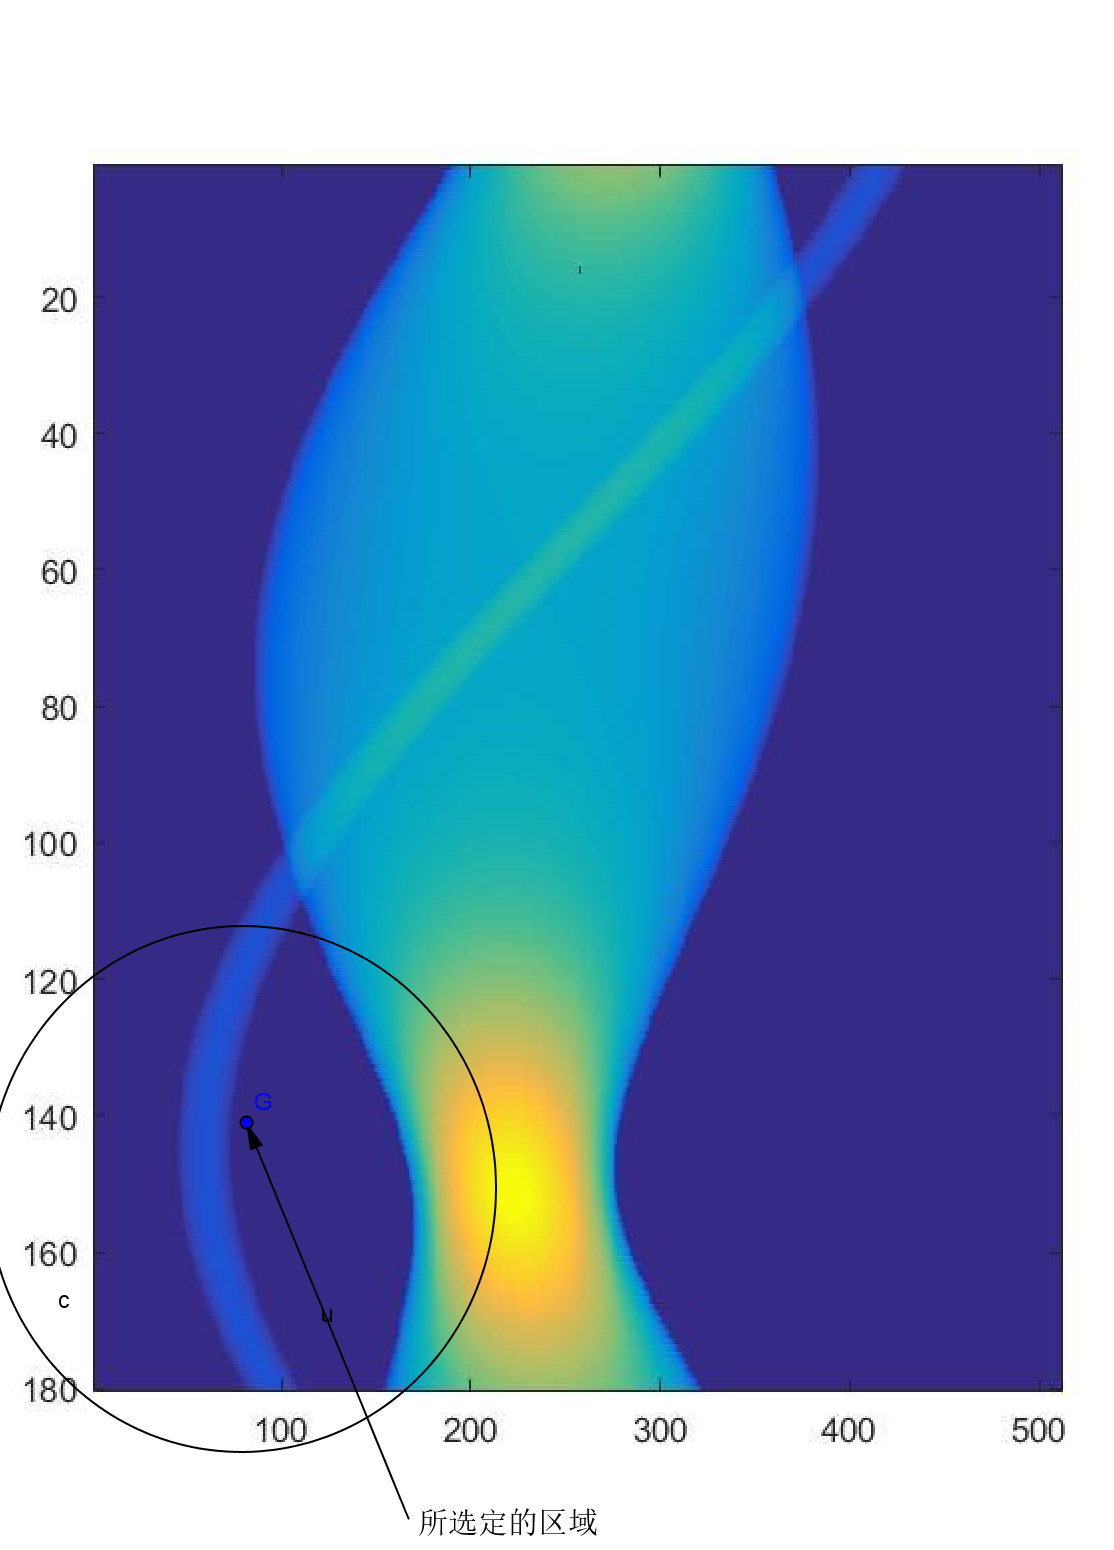
\includegraphics[width=.6\textwidth]{2.png}
\caption{取值领域示意图}
\end{figure}
\par
取G的区域是为了避免选取到椭圆的吸收率数据,否则比例将不成立。

此时,可用小圆的直径比数据中每一列不为0的行总个数,就可得出以下比例:
\begin{equation}
\frac{ D_2}{D^{'}_{2}} = \frac{\ell }{1} 
\end{equation}
其中$D^{'}_{2}$为每一行不为0的总个数。
另外,知道CT是根据衰减系数来决定其吸收率[1],因此引入公式
\begin{equation}
A=A_0e^{{\mu}x}
\end{equation}
其中A为衰减后的数值,$A_0$为初始数值。
结合所给出的数据,可将(2)转化为以下形式。先选定最长距离,知其对应的吸收率是最高的。
因而有:
\begin{equation}
{\mu}d_{max}=P_{max}
\end{equation}

设CT的X射线从PQ方向射出
\begin{figure}[H]
\centering
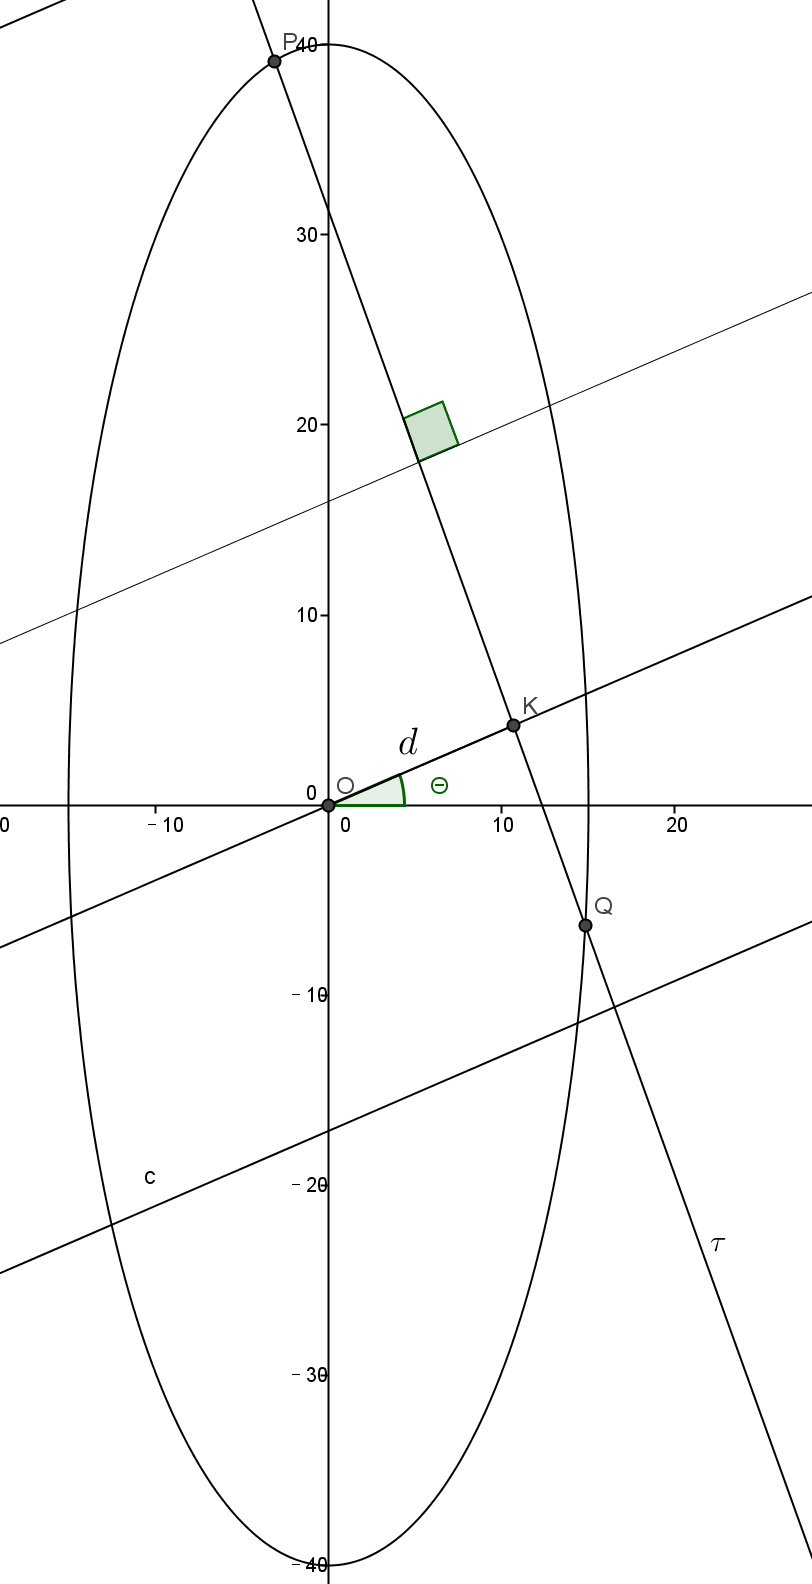
\includegraphics[width=.6\textwidth]{3.png}
\caption{椭圆圆心建系图}
\end{figure}
其中$d=OK$,
设椭圆的密度值为$\rho$,从投影值的定义可知:
\begin{equation}
P=\int_{PQ}{\rho}\mathrm{d}l={\rho}PQ
\end{equation}
而椭圆的方程为:
\begin{equation}
(\frac{x}{15})^2+(\frac{y}{40})^2=1
\end{equation}
射线PQ的法线式为
\begin{equation}
x\cos{\theta}+y\sin{\theta}=d
\end{equation}
从(5),(6)中可解出射线与椭圆交点P,Q的坐标
因而可以得到PQ的长度:
\begin{equation}
PQ=\frac{2 \times 15\times 40\sqrt{r^2-d^2}}{r^2}
\end{equation}
其中
\begin{displaymath}
r^2=(15\cos{\theta})^2+(40\sin{ \theta})^2
\end{displaymath}
根据(4),可得出以下方程组
 \begin{equation}
\left\{
\begin{array}{rl}
{\mu}PQ&=P_1\\

{\mu}P^{'}Q^{'}&=P_2\\
\end{array}
\right.
\end{equation}
另外,我们知道每一条射线对应的投影值与第i个探测器有关,利用上述求出的$\ell$,可化为
\begin{equation}
PQ=\frac{2 \times 15\times 40\sqrt{r^2-d+kl{\ell}^2}}{r^2}
\end{equation}

知旋转中心的特征为:在图中,在第256和257之间的检测器必然穿过去
\subsubsection {模型的解决}
通过(1)的公式,再计算出平均数值,得出
$$\ell \approx 0.2775  mm$$
进而我们得知$\ell$的值
通过(3),可估计出$\mu$的数值。
\begin{displaymath}
\mu \approx 1.7721
\end{displaymath}

再利用(6),(8),(9)求出每次转动的角度。
求得
\begin{displaymath}
\theta_i-\theta_{i-1} \approx 1.0003°,i=2,\dots,179
\end{displaymath}
这个结果符合了每一次实验转动180度求解的必要条件,视为可接受的误差值。

\section{问题二的分析}
\subsubsection {模型的建立}
对于问题二,本题附件三中给出了不同角度下,各个探测器的接收情况,通过这些数据我们需要求解出新的介质的位置,几何形状以及各点吸收率的情况。我们选择用matlab自带的iradon函数将其求出,将利用问题一所求出的数据进行反投影建模。在Matlab里成功实现。
\subsubsection {模型的解决}
\begin{figure}[H]
\centering
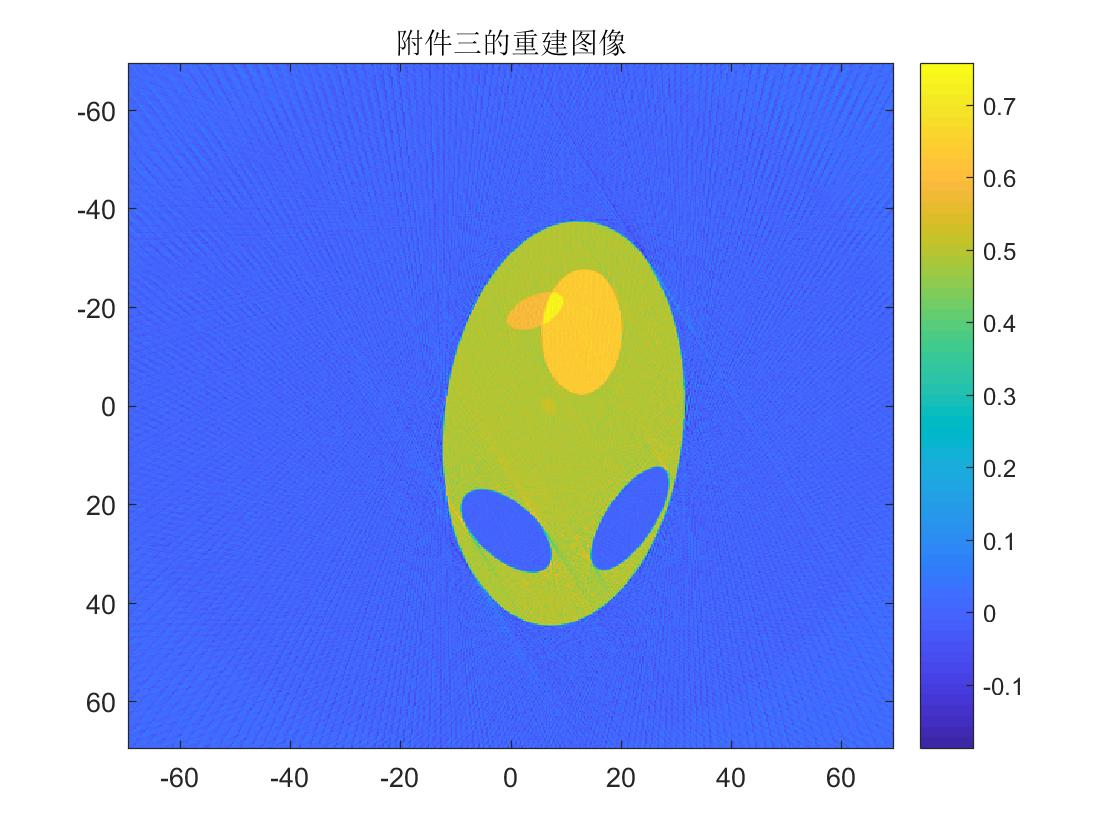
\includegraphics[width=.6\textwidth]{7.jpg}
\caption{问题二的反投影模型}
\end{figure}
所求出的十个点为
\begin{center}
\begin{tabular}{|c|c|c|c|c|c|c|c|c|c|c|}
 \hline
x    &  10   & 34.5   &  43.5       &  45          &  48.5        &  50           &  56          &  65.5      &  98.5   &  43.5\\ \hline 
y    &    18 &  25    &  33           &  75.5        &  55.5       &  75.5        &  76.5       &  37      &  18   &  43.5   \\ \hline
p    &   0    &  0      &  0.4918   &  0.4814   &  0.4858   &  0.0310   &  0.0081   &  0       &  0   &  0.00318\\ \hline
\end{tabular}
\end{center}


\section{问题三的分析}
\subsubsection {模型的建立}
对于问题三,与问题二有些许相似,于是采用同样方法求解,但求出的图像不像第二问样规则,是极其不规则的图形,修正后也无法辨别10个点的吸收率。于是在修正后,为了精确求得10个点的吸收率,我们选择采用滤波反投影重建算法而不直接调用iradon函数来求解。
因为反投影算法会产生星状伪迹,重建后的图像边缘模糊不清,因此调用滤波函数来尽可能消除星状伪迹的影响。

\begin{figure}[H]
\centering
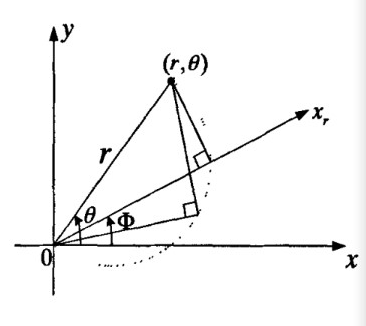
\includegraphics[width=.6\textwidth]{5.png}
\caption{卷积反投影}
\end{figure}
\subsubsection {模型的解决}
\begin{figure}[H]
\centering
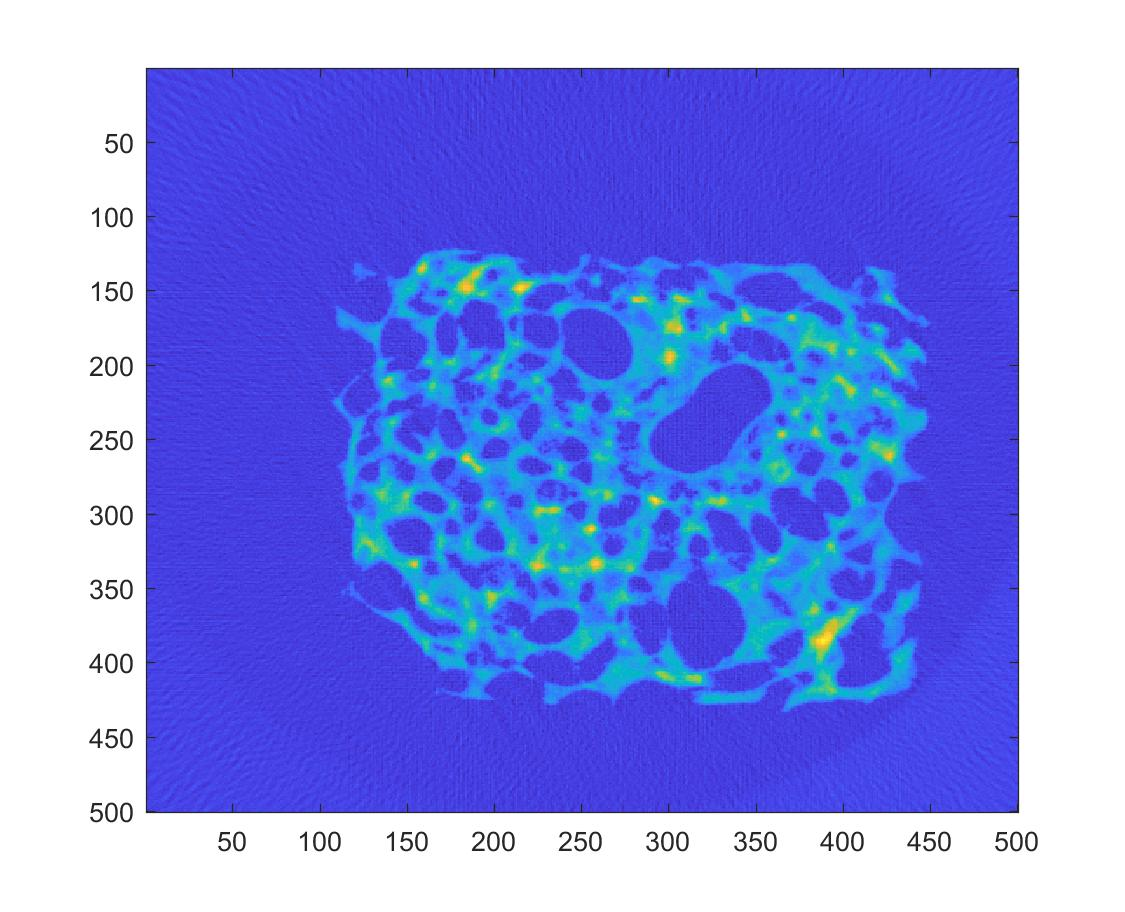
\includegraphics[width=.6\textwidth]{8.jpg}


以上为问题三的二维图。
所求出对应的十个点为
\begin{center}
\begin{tabular}{|c|c|c|c|c|c|c|c|c|c|c|}
 \hline
x    &  10   & 34.5   &  43.5       &  45          &  48.5        &  50           &  56          &  65.5      &  98.5   &  43.5\\ \hline 
y    &    18 &  25    &  33           &  75.5        &  55.5       &  75.5        &  76.5       &  37      &  18   &  43.5   \\ \hline
p    &   2.0741   &  0.4251      &0.9073   &  0.4814   & 0.4090   & 0.0237 & 3.2771   &  0.7881       &  0   &  0.00318\\ \hline
\end{tabular}
\end{center}
\end{figure}
\section{问题四的分析}
\subsubsection {模型的解决}
造成这题中的误差来源于星状伪迹,也就是吸收率p存在误差,而p的误差delta p来源于
光线的入射角度a,物体所在位置的距离r(相对原点)和角度b【极坐标下的情况】,而p的误差会造成线积分时p(x,y)的偏差,从而对最后的结果产生影响。
为了深一步了解其误差含义,我们调用IRadon函数来对问题一的模型进行反投影建模。再与原本的数据给出的图进行对比。
\begin{figure}[H]
\centering
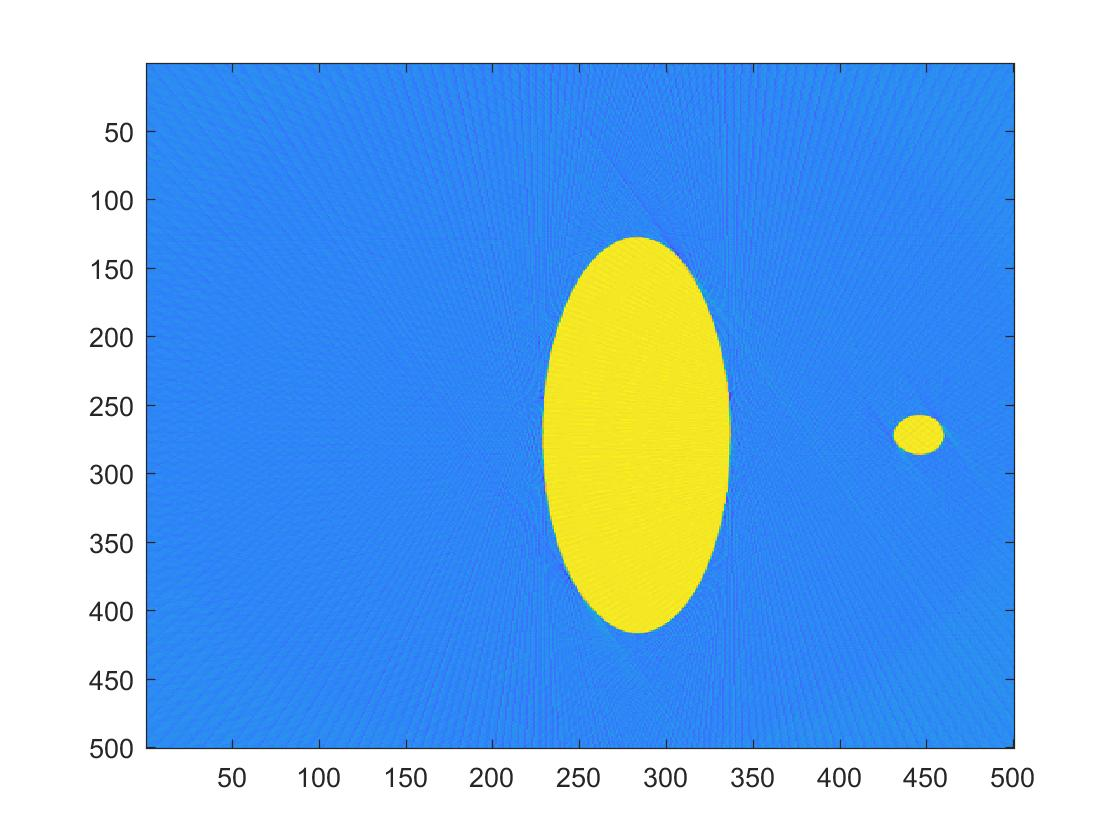
\includegraphics[width=.6\textwidth]{6.jpg}
\caption{问题一的反投影模型}
\end{figure}

\begin{figure}[H]
\centering
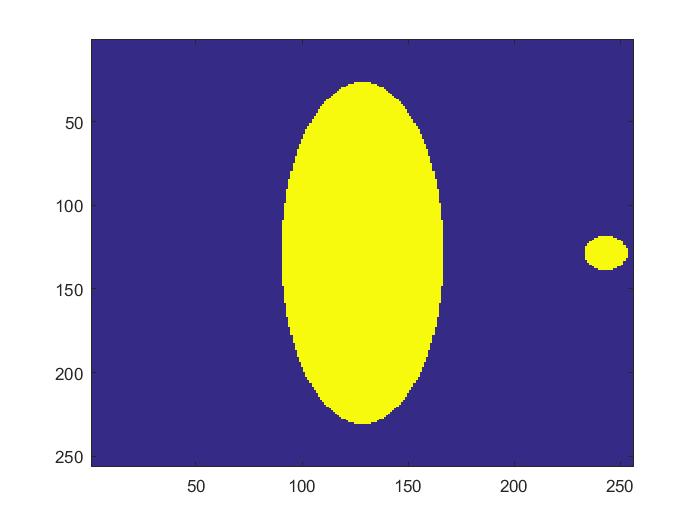
\includegraphics[width=.6\textwidth]{9.jpg}
\caption{问题一数据所给出的模型}
\end{figure}
在两张图上,分析出来的是位置上出现明显区别,但
其绘制表格的代码及其说明如下。


 
%参考文献
\begin{thebibliography}{9}%宽度9
 \bibitem{bib:one} 庄天戈. CT原理与算法  上海交通大学出版社 , 1992
 \bibitem{bib:two} 范慧赟.CT图像滤波反投影重建算法的研究  西北工业大学硕士论文 ,2007
 \bibitem{bib:three} 冯开梅. 医学影像设备人民卫生出版社, 2008
 \bibitem{bib:four}  郭炳映.CT实验平行束投影与反投影重建报告,2012
\end{thebibliography}

\newpage
%附录
\appendix
 \section{解出每两个检测器单元的距离--matlab源代码}
\begin{lstlisting}[language=matlab]
clc, clear
data1=xlsread('problem1_2.xls');
data1 = data1';
array = [];
for i = 110:180
    num = 0;
    for j = 1:110
        if (data1(i,j) ~= 0)
            num = num + 1;
        end
    end
    if (num ~= 0)
        array = [array num];
    end
    sd=sum((array-28.82882883))
end

% 探测器单位距离=0.2775
l = 8/mean(array)
 \end{lstlisting}
\section{计算角度差值--matlab 源程序}
\begin{lstlisting}[language=matlab]
clc, clear
data1=xlsread('problem1_2.xls');
a = 40; % 半长轴
b = 15;  % 半短轴
data1 = data1';
d = 8;  % 直径
l = 0.2775; % 探测器单位距离

array = [];
for i = 110:180
    array2 = [];
    for j = 1:110
        if (data1(i,j) ~= 0)
            array2 = [array2 data1(i, j)];
        end
    end
    array = [array max(array2)];
end

Pmax = mean(array);
miu = Pmax/d

% 每一排选两个探测器
thetas = [];
for i = 90:180
    j = 225;
    save('var1')
    theta = get_theta(data1(i,j), data1(i,j+5), 5);
    thetas = [thetas theta];
end

% 计算角度的差值
delta = [];
for i = 1:90
    delta = [delta abs(thetas(i+1)-thetas(i))];
end
delta_mean = mean(delta)*180/pi;
 \end{lstlisting}
\section{滤波反投影--matlab 源程序}
\begin{lstlisting}[language=matlab]
clc, clear
% 加载数据数据
x0 = 50-9.2963;
y0 =  50 + 5.5500;
l = 0.2775;
M = 512;
delta = 1.001;

p = xlsread('sheet3.xlsx');
p = p';
pfilter = p;

disp('开始滤波')
filternum=128;
filter_ramp=zeros(filternum,1);
for j=1:filternum   % 16 point ramp filter
    i=j-1-filternum/2;
    if(i==0)
     filter_ramp(j,1)=1/(8.0);
    elseif (mod(i,2)==0)
            filter_ramp(j,1)=0;
    elseif (mod(i,2)==1)
            filter_ramp(j,1)=-0.5/(i*i*pi*pi);
    end
end
m=1;
figure(4);

plot(filter_ramp);


pfilter=[];
length_conv=filternum+512-1;%639
pPro=zeros(length_conv,1);
temp_pro=zeros(512,1);
h_filter=filternum/2;%64
ii=length_conv-h_filter-512;%63
 for s=1:180 % sample-loop
    % for  pp=1:h_filter
    pro_left =(p(s,1)+p(s,2))/2.0;
    pro_right=(p(s,512)+p(s,512-1))/2.0;
    
    for pp=1:h_filter               %left part
        pPro(pp,1)=pro_left;  %左边补零      
    end
%    
    for pp=1:512                      %middle part
     pPro(h_filter+pp,1)=p(s,pp);%中间部分不变
    end
%    
   for pp=h_filter+512+1:length_conv
    pPro(pp)=pro_right;%右边补零
    end
%   result_conv    
   for n=1:512 
       result_conv=0;
   	for jj=1:filternum%1:128
        pPmove=pPro(n+jj-1,1);
        result_conv=result_conv+pPmove*filter_ramp(jj,1);
    end
    pfilter(s,n)=result_conv;
   end
 
    
 end
figure(5);
showimge(pfilter,180,512,min(min(pfilter)),max(max(pfilter)));%输出卷积滤波结果

rou = [];
for i = 1:100
    x = abs(i - x0);
    for j = 1:100
        y = abs(j - y0);
        r = sqrt(x^2+y^2);
        theta = atan(y/x);
        P = 0;
        for m = 1:179
            P_sum = 0;
            phi = m*delta + 30;
            if phi > 180
                phi = phi - 180;
            end
            nlambda = ((1+M*l)/2 + y*sin(theta - phi) + x*cos(theta-phi))/l;
            if nlambda > 511 || nlambda < 0
                P = 0;
            else
                n = floor(nlambda);
                lambda = nlambda - n;
                P = (1-lambda)*pfilter(m,n+1) + lambda*pfilter(m, n+2); %插值
            end
            P_sum = P_sum + P;
        end
        rou(i,j) = P_sum/180;
    end
end
            
        
        =
 \end{lstlisting}


\end{document} 
